\section{Evaluation}
\label{sec:eval}

This section evaluates the mask--product--merge pipeline developed in
this chapter. It proceeds in four parts. After describing the
experimental setup, we first compare the three mask-creation
strategies of Section~\ref{subsubsec:fast-intersection} in isolation,
then benchmark the full pipeline end to end against the reference
continuous-tensor implementation in Finch, and finally break the
end-to-end time into its three stages to see where the time goes.

\subsection{Experimental Setup}
\label{subsec:eval-setup}

\paragraph{Hardware.}
All experiments run on a single machine with an Intel Core i9-10900K
CPU (10 cores, 20 hardware threads, 3.70\,GHz) with 125\,GB of RAM,
and an NVIDIA GeForce RTX~3090 GPU with 24\,GB of memory.

\paragraph{Implementation.}
We implement the pipeline in PyTorch (version 2.9), exactly as in the
listings of this chapter: the mask, product, and merge steps are
composed from broadcast comparisons, gathers, scatter-adds, sorts, and
flat \texttt{unique} calls, so the same code runs unchanged on CPU and
GPU. The dense and binary-search mask builders are PyTorch; the
database-join builder runs on Polars (version 1.35), using its GPU
engine when the pipeline runs on the GPU. Unless stated otherwise, the
end-to-end pipeline uses the binary-search builder. We evaluate three
configurations of our implementation: \emph{CPU-single} (one thread),
\emph{CPU-multi} (all 20 threads), and \emph{GPU}.

\paragraph{Baseline.}
We compare against the original implementation of continuous tensors,
an extension of the Finch compiler~\cite{finch}, which generates
single-threaded CPU code in Julia. Finch does not operate on COO
inputs: each operand must first be converted into Finch's nested
run-length (SparseRLE) levels, and multi-dimensional interval operands
must additionally be fragmented at the outer dimension's endpoints to
make the nesting disjoint. Because our pipeline consumes COO directly
while Finch requires this separate format, the full benchmark reports
Finch's format-conversion time alongside its kernel time; Finch's
one-time kernel compilation is excluded, as it is amortizable across
runs.

\paragraph{Notation.}
Each benchmark is written as an Einsum whose superscripts give the
coordinate type of every dimension: $P$ for a pinpoint dimension and
$I$ for an interval dimension. For example,
$C^{I}_{x} = \int_r A^{II}_{xr}\, B^{I}_{r}\, dr$ is a matrix--vector
contraction in which every dimension of every operand is an interval.
All intervals in this evaluation are half-open, $[s, e)$.

\paragraph{Dataset.}
We use synthesized operands: each operand's $n$ pieces are sampled
without replacement from a regular grid of roughly $2n$ cells over
$[0, 64)^{D}$, with each piece's intervals (or pinpoints) drawn inside
its own cell, so that two operands generated from different seeds
interact exactly where their sampled cells collide. A skew parameter
in $[0, 1]$ biases the sampling toward one corner of the grid, which
controls how many pieces of the two operands interact; unless noted,
we report skew $0.5$, and piece values are drawn uniformly from
$[0.5, 1.5)$. Every measurement is the median of five timed runs after
two warmup runs (the first warmup absorbs \texttt{torch.compile}
overhead), with the GPU synchronized around every timed region.

\subsection{Comparing Mask-Creation Strategies}
\label{subsec:eval-mask}

\begin{figure}[t]
\centering
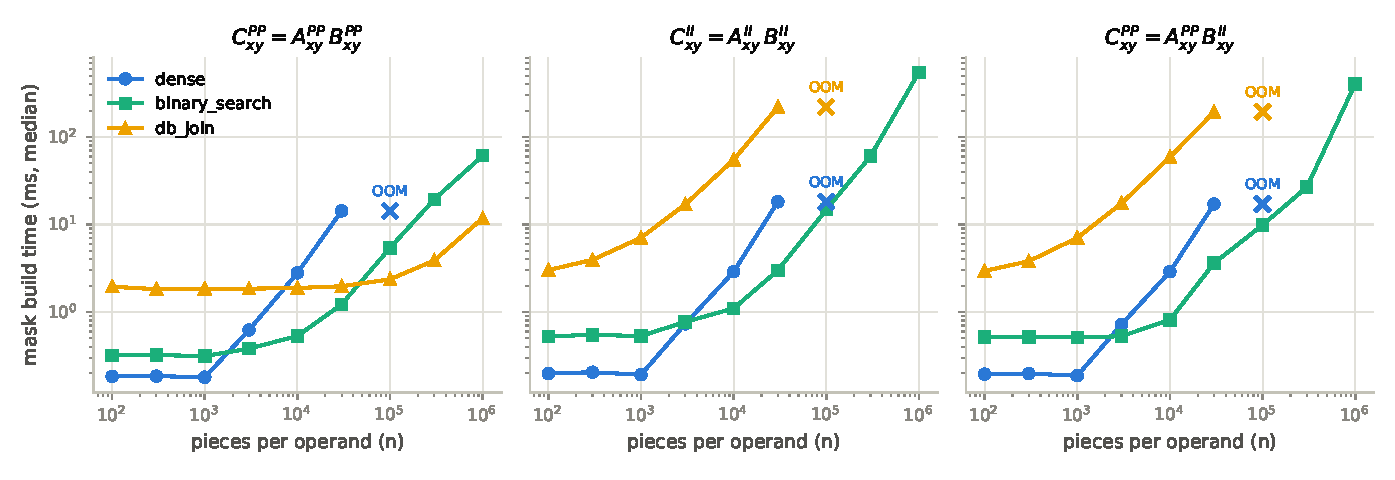
\includegraphics[width=\textwidth]{figures/exp1_summary.pdf}
\caption{Mask creation on the GPU: the three builders of
Section~\ref{subsubsec:fast-intersection} on the three join types, as
the number of pieces $n$ grows (log--log). Left: composite equality
(all pinpoints). Middle: interval--interval overlap. Right: mixed
point-in-box. A line ends where the builder fails (out of memory or
guarded out).}
\label{fig:eval-exp1}
\end{figure}

Figure~\ref{fig:eval-exp1} compares the three mask builders on the
GPU, on the three kinds of join condition a continuous Einsum
generates: pure \emph{equality} joins, where every shared dimension is
a pinpoint on both operands; pure \emph{inequality} joins, where every
shared dimension is an interval on both operands and the condition is
the pair of overlap inequalities of Section~\ref{subsec:cont-mask};
and the \emph{mixed} case of a pinpoint operand against an interval
operand, a point-in-box test. All three builders produce identical
masks; only the time differs. Three findings stand out.

First, \emph{the dense table wins at small $n$}. Up to a few thousand
pieces the broadcast comparison is a single fused kernel with no sort
and no data-dependent control flow, and the GPU absorbs the $n^2$
table without effort: at $n = 1{,}000$ the dense builder takes about
$0.2$\,ms on every case, ahead of binary search ($0.3$--$0.7$\,ms) and
far ahead of the database join ($2$--$7$\,ms, dominated by fixed
engine overhead). The quadratic table is also what ends it: the dense
builder is the first to hit the memory wall and is guarded out beyond
$n \approx 10^{4}$--$10^{5}$.

Second, \emph{the database join is excellent on equality joins and
poor on inequality joins}. Equality joins are the case database
engines are built for: Polars executes them as hash joins, and on the
all-pinpoint case it overtakes binary search at large $n$
($11.9$\,ms versus $61.3$\,ms at $n = 10^{6}$). Inequality joins
invert the picture. \texttt{join\_where} cannot use a hash table for
the overlap inequalities and falls back to a far more expensive plan:
on the 1-D interval-overlap case it is over $100\times$ slower than
binary search at $n = 10^{5}$ ($757$\,ms versus $5.3$\,ms), and on the
2-D interval cases it fails outright at that size.

Third, \emph{binary search is the robust middle ground}. It is never
the fastest at small $n$ and it loses the largest equality joins to
the hash join, but it is the only builder that completes every case at
every size, and on the interval-overlap joins, the common case for
continuous Einsums, it is the fastest at every $n$ beyond the dense
builder's reach. This is why it is the default builder in the full
benchmark that follows.

\subsection{Full Benchmark}
\label{subsec:eval-full}

\begin{table}[t]
\centering
\caption{The seven Einsums of the full benchmark. Superscripts give
each dimension's coordinate type ($P$ pinpoint, $I$ interval);
$\int$ marks a contraction over a continuous variable.}
\label{tab:eval-cases}
\small
\begin{tabular}{lll}
\toprule
Case & Einsum & Description \\
\midrule
pointwise 1-D &
$C^{I}_{x} = A^{I}_{x}\, B^{I}_{x}$ &
elementwise product of interval vectors \\
pointwise 2-D &
$C^{II}_{xy} = A^{II}_{xy}\, B^{II}_{xy}$ &
box--box intersection (Example~1) \\
diagonal &
$C^{I}_{x} = A^{II}_{xx}\, B^{I}_{x}$ &
diagonal extraction times a vector \\
matrix--vector &
$C^{I}_{x} = \int_r A^{II}_{xr}\, B^{I}_{r}\, dr$ &
contraction, 1-D output (Example~2) \\
matrix--matrix &
$C^{II}_{xy} = \int_r A^{II}_{xr}\, B^{II}_{ry}\, dr$ &
contraction, 2-D output \\
triple contraction &
$D^{PP}_{xy} = \int_r A^{PP}_{xy}\, B^{II}_{xr}\, C^{II}_{ry}\, dr$ &
three operands, mixed types \\
box search &
$C^{PP}_{xy} = A^{II}_{xy}\, B^{PP}_{xy}$ &
one query box against $n$ points \\
\bottomrule
\end{tabular}
\end{table}

\begin{figure}[t]
\centering
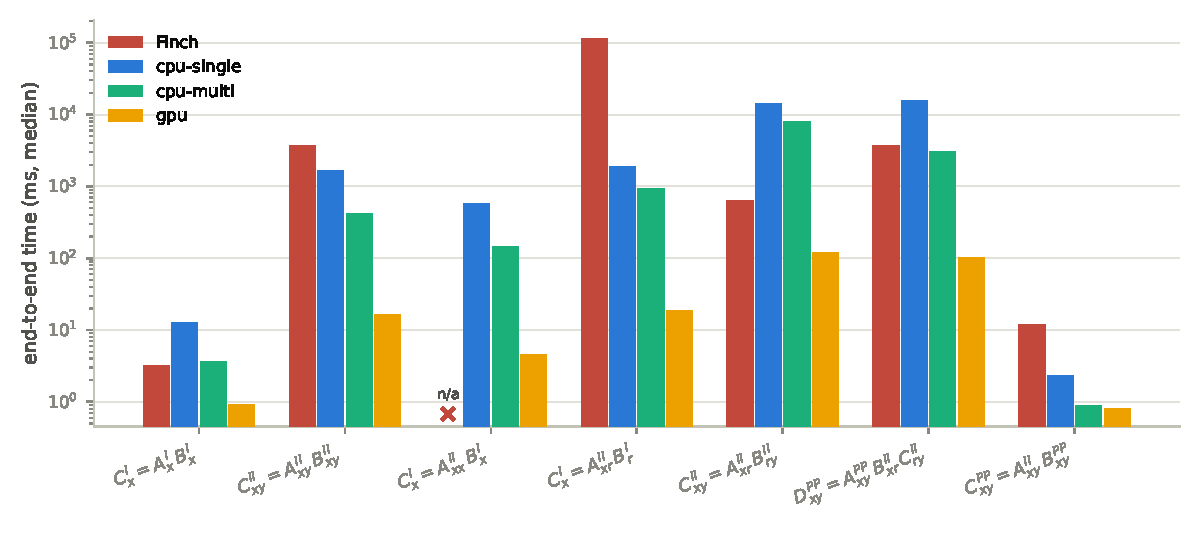
\includegraphics[width=\textwidth]{figures/exp2_summary.pdf}
\caption{End-to-end time of the seven Einsums of
Table~\ref{tab:eval-cases} at $n = 10^{5}$ pieces per operand
(log scale). The Finch bar stacks the COO-to-Finch format conversion
on top of the kernel time; the diagonal case is n/a for Finch.}
\label{fig:eval-exp2}
\end{figure}

Table~\ref{tab:eval-cases} lists the seven Einsums of the full
benchmark. They are chosen to cover the axes along which the pipeline
varies: with and without a contraction, one to three operands, 1-D and
2-D outputs, and pinpoint, interval, and mixed coordinate types. For
the matrix--matrix contraction the operands' intervals are aligned to
the grid cells of the generator; with free endpoints the contraction's
exact piecewise output grows towards the full $(2n)^{2}$ breakpoint
grid, on the order of $10^{10}$ pieces at this scale, which no
implementation could materialize. (The stage breakdown of
Section~\ref{subsec:eval-breakdown} measures exactly this blow-up at
smaller sizes.)

Figure~\ref{fig:eval-exp2} shows all seven cases at $n = 10^{5}$
pieces per operand, comparing Finch against our implementation in its
CPU-single, CPU-multi, and GPU configurations. All four start from the
same COO data; the Finch bar additionally stacks the format-conversion
time discussed in Section~\ref{subsec:eval-setup}, which is far from
negligible: fragmenting a 2-D interval operand at its outer endpoints
turns the $10^{5}$ input pieces into roughly $3.3 \times 10^{7}$
run-length fragments, and the conversion alone ($3.2$\,s) exceeds
Finch's own kernel time on the pointwise 2-D case ($0.58$\,s). The
diagonal case is marked n/a for Finch: the repeated index in
$A^{II}_{xx}$ does not lower through Finch's nested continuous levels,
so no Finch kernel exists for it.

Comparing kernel times at equal parallelism, one thread each,
\emph{Finch often beats our CPU pipeline}. Its generated code streams
through the sorted operands and merges them in place, where our
pipeline materializes the mask and candidate arrays and pays for
sorts; on the matrix--matrix contraction Finch needs $0.61$\,s where
CPU-single needs $14.4$\,s. The comparison is not uniform: on the
matrix--vector contraction the roles reverse dramatically ($112$\,s
for Finch versus $1.9$\,s for CPU-single), and once the stacked
conversion cost is counted, our single-thread pipeline is also ahead
on the pointwise and triple-contraction cases. CPU-multi accelerates
our pipeline by a further $2$--$5\times$, which still does not
consistently overtake Finch's kernels.

\emph{The GPU changes the conclusion.} Every step of the pipeline is a
data-parallel primitive, so the same code that loses on one CPU thread
runs $100$--$155\times$ faster on the GPU for every large case, and
the GPU configuration wins every benchmark outright. Against Finch's
kernel plus conversion, the GPU pipeline is $5.4\times$ faster on the
contraction Finch handles best (matrix--matrix, $119$\,ms versus
$0.64$\,s) and two to three orders of magnitude faster elsewhere
(e.g.\ pointwise 2-D, $16.6$\,ms versus $3.8$\,s). This is the central
result of the chapter: reformulating continuous Einsums as
mask--product--merge makes them run entirely on primitives a GPU
executes well, which the pointer-chasing loops of the sequential
formulation cannot.

\subsection{Stage Breakdown}
\label{subsec:eval-breakdown}

\begin{figure}[t]
\centering
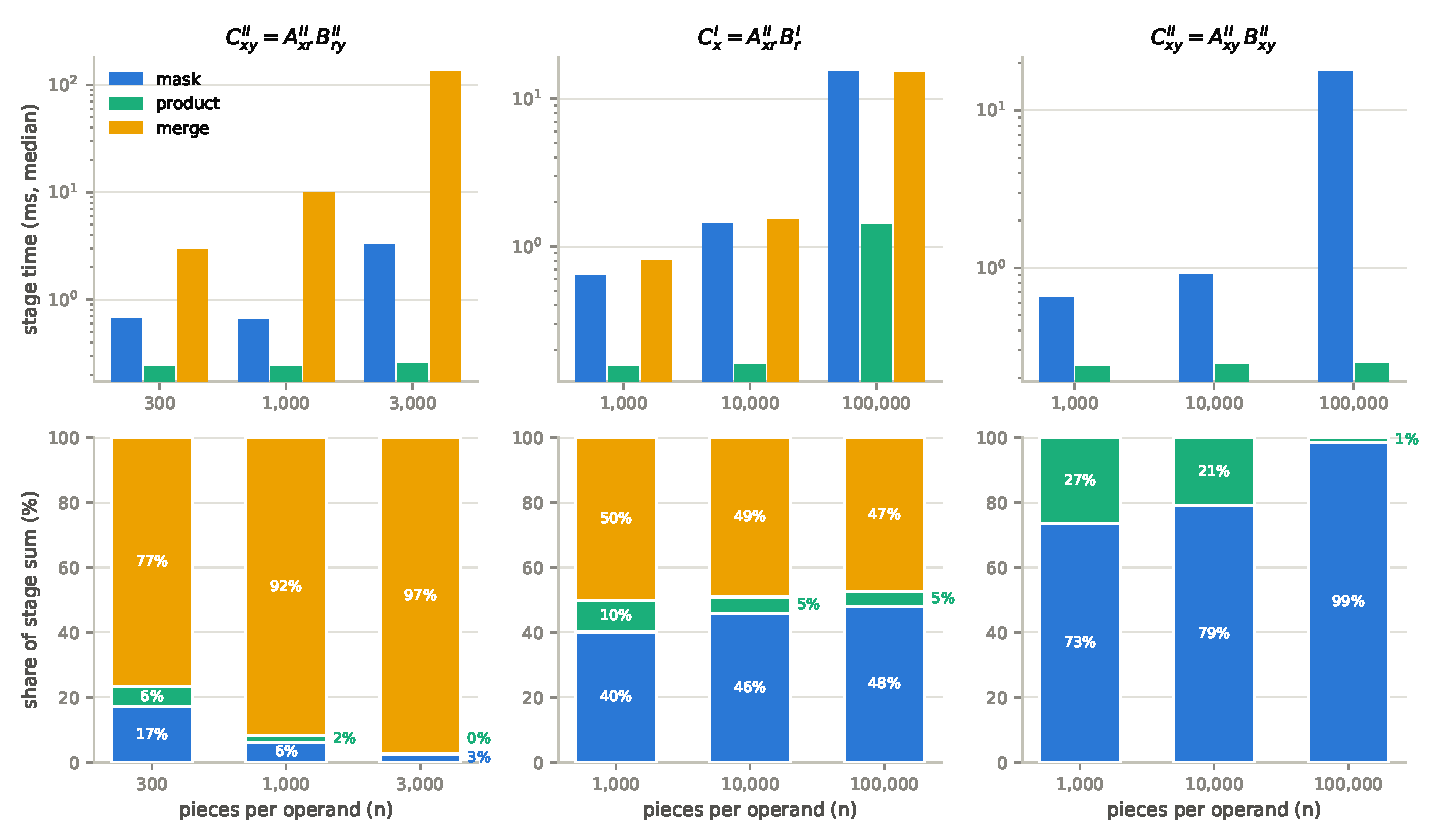
\includegraphics[width=\textwidth]{figures/exp3_stages.pdf}
\caption{GPU time per pipeline stage for three representative cases as
$n$ grows. Mask creation and merge dominate; the product step is
negligible throughout. The matrix--matrix case uses free (unaligned)
interval endpoints and is swept only to $n = 3{,}000$: its merged
output already reaches $2.6 \times 10^{7}$ pieces there, and larger
sizes exhaust GPU memory.}
\label{fig:eval-exp3}
\end{figure}

Finally, Figure~\ref{fig:eval-exp3} splits the GPU pipeline into its
three stages on three representative cases: the pointwise 2-D product
(no contraction), the matrix--vector contraction (a contraction whose
output stays small), and the matrix--matrix contraction with free
interval endpoints (a contraction whose output explodes). Together
they show that the pipeline has exactly two costs, and which one you
pay is a property of the Einsum.

Without a contraction, \emph{mask creation is essentially the whole
pipeline}: on the pointwise 2-D case at $n = 10^{5}$, mask creation
takes $17.6$\,ms of the $17.7$\,ms total, the product step is a few
gathers ($0.2$\,ms), and no merge is needed because the candidates are
already disjoint (Section~\ref{subsec:cont-merge}). With a
contraction, the merge appears and can grow to match or dominate the
mask. On the matrix--vector case the two split the time almost evenly
($15.2$\,ms mask, $15.0$\,ms merge at $n = 10^{5}$): the mask yields
$1.0 \times 10^{7}$ candidates that the merge condenses into
$1.9 \times 10^{5}$ output pieces. On the free-endpoint matrix--matrix
case the merge takes over completely, $132$\,ms of the $174$\,ms total
already at $n = 3{,}000$, because the cut step of
Section~\ref{subsec:cont-merge} must replicate every candidate across
the segments it covers and the output itself explodes; this is the
memory blow-up that forced the aligned operands in the full benchmark,
and it is inherent to the problem (the exact piecewise output really
has that many pieces), not to the method.

The breakdown justifies the design effort of this chapter: the product
step, the only part that touches the operand values, is never the
bottleneck. All the time is in mask creation, which
Section~\ref{subsec:eval-mask} showed is best served by different join
strategies in different regimes, and in the merge, whose rank-space
formulation is what keeps it a composition of sorts, prefix sums, and
scatter-adds that the GPU executes at full throughput.
